% STATUS: SSOT -- motion control gain estimation, running record (started 2026-10-05 from motion_ctrl.pptx + 1004_q55_ratio_from_kf.tex).
% ======================================================
% Compile: xelatex motion_ctrl.tex (our version) and xelatex motion_ctrl_share.tex (for others)   (from reference/eq17_analysis/derivation/)
% Parts (one \input file each, so the two sessions on this work tree edit different files):
%   motion_ctrl/part0_status.tex        settings in force, change log, open items        (main editor: ap model session)
%   motion_ctrl/sec1_model.tex          S1 discrete-time motion model and control law (normalized; paper II-D)   (Layer-1, 10-07)
%   motion_ctrl/sec2_gain.tex           S2 effect of the motion gain on tracking (paper Fig. 5, three axes)    (Layer-1, 10-07)
%   motion_ctrl/sec3_am.tex             S3 measured input gain (paper II-E)                                    (Layer-1, 10-07)
%   motion_ctrl/sec4_estimator.tex      S4 augmented estimator, first order (paper II-F)                       (Layer-1, 10-07)
%   (motion_ctrl/archive/part1_first_order.tex = the old S4, lambda_c 0.7, no longer input)
%   motion_ctrl/sec5_conly.tex          S5 position-dependent motion gain, c-only, q55 = 0, plane      (Layer-1, 10-07)
%   motion_ctrl/sec6_wall.tex           S6 unknown wall type (plane, cell), q55 = P_fix^2 I               (Layer-1, 10-07)
%   motion_ctrl/sec7_raster.tex         S7 reference result: raster scan parallel to the wall              (Layer-1, 10-07)
%   (motion_ctrl/archive/part2_conly.tex = the old c-only part, w notation, no longer input)
% Restructure in progress (user 10-07): outline and notation in motion_ctrl/PLAN_notation_outline.md.
%   motion_ctrl/appendix_figures.tex    figure provenance: figure <- plot script <- runs
% Rules: equations, section titles, one setting line per figure page; no readings (derivation-workflow rule 10, 0924 report convention).
%   Every figure page = one trajectory, seed 1, rows a_bar | e_a | delta_x_m [um] (| c). Regenerate all figures:
%   test_script/scratch/make_motion_ctrl_figs.m. Tex and the figures it includes go in the same commit (matlab-conventions).
% Preamble copied from 1004_q55_ratio_from_kf.tex.
% ======================================================
\documentclass[11pt,a4paper]{ctexart}
\usepackage[fleqn]{amsmath}
\usepackage{amssymb,bm}
\usepackage{graphicx}
\usepackage{booktabs}
\usepackage{array}
\newcolumntype{L}[1]{>{\raggedright\arraybackslash}p{#1}}
\graphicspath{{figures/}}
\setlength{\mathindent}{0pt}
\usepackage{geometry}
\geometry{margin=2.2cm}
\setlength{\parindent}{0pt}
\setlength{\parskip}{0.2em}
\setlength{\abovedisplayskip}{6pt}
\setlength{\belowdisplayskip}{6pt}
\setlength{\abovedisplayshortskip}{6pt}
\setlength{\belowdisplayshortskip}{6pt}
\newcommand{\lc}{\lambda_c}
\newcommand{\bx}{\bar{x}}
\newcommand{\ba}{\bar{a}}
\newcommand{\bw}{\bar{w}}
\newcommand{\ap}{\ba'}
\newcommand{\wh}{\hat{\bw}}
\newcommand{\hh}{\hat{h}}
\newcommand{\ch}{\hat{c}}
\newcommand{\Pf}{p^{f}_{55}}
\newcommand{\Pu}{p_{55}}
\newcommand{\Pfix}{p_{\mathrm{fix}}}
\newcommand{\hd}[1]{\par\bigskip\noindent\underline{\textbf{#1}}}
% one figure page: title, one setting line, the figure
\newcommand{\figpage}[3]{\clearpage\subsection*{#1}\noindent{\small\textcolor[gray]{0.35}{#2}}\par\smallskip
  \begin{center}\includegraphics[width=\textwidth,height=0.82\textheight,keepaspectratio]{#3}\end{center}}
\usepackage{xcolor}
\pagestyle{plain}

\begin{document}

% Two versions (user 10-05): this file = our version (status page + appendix); motion_ctrl_share.tex sets \mcshare
% and gives the version for others (body only, no status page, no appendix).
\begin{center}
{\Large\textbf{Motion control: gain estimation}}
\ifdefined\mcshare\else\\[0.4em]{\small running record, started 2026-10-05}\fi
\end{center}

\ifdefined\mcshare\else% Part 0 of motion_ctrl.tex: settings in force, change log, open items. Settings only (no readings).
\section*{Status}

\hd{Settings in force}

\smallskip
{\small
\begin{tabular}{@{}L{2.0cm}L{8.6cm}L{5.0cm}@{}}
\toprule
item & setting & where \\
\midrule
notation & normalized: $\bx = x/R$, $\ba = a_x/a_{nom}$, $\bar f = a_o f$; wall surface at $\bx = 0$; paper wording (Meng TIE 2025) & \texttt{motion\_ctrl/PLAN\_notation\_outline.md} \\
$\lc$ & 0.4 for every figure (the paper's value; all sections rerun 10-07) & \texttt{run\_plaw\_walls} \texttt{opts.lambda\_c} \\
Section 2 & three axes; $x_d = y_d = 9\sin(2\pi t)$ \textmu m, $z_d$: 50 $\to$ 2.475 \textmu m (22.2 $\to$ 1.10 R) in 5 s, the z height of the later sections; law with $\hat{\ba} = \ba$ or $1$ & \texttt{run\_mc\_s2\_xyz.m} \\
trajectory & $\bw$: $22.2 \to 1.10$ constant-velocity descent in $T_d$, then triangle $1.10 \leftrightarrow 2.00$ for 2 s at $f$; no hold & \texttt{canonical\_scenario 'ramp\_tri'} \\
\quad defaults & $T_d = 1$ s, $f = 1$ Hz (canonical); figures: $T_d = 0.5$ s with the triangle, $T_d = 2$ s descent only & \texttt{run\_plaw\_walls} \texttt{opts.Td}, \texttt{opts.f\_osc} \\
walls & plane (estimator init), cell = plane slid down 1.05 R (plant only) & \texttt{cell\_cperp\_delta.m} \\
figures & seed 1; rows $\ba$ $|$ $e_{\ba}$ $|$ $\delta x_m$ [µm] ($|$ $c$) & \texttt{plot\_5state\_noap\_rtri}, \texttt{plot\_conly\_rtri\_final} \\
first order & $Q_{44}[k] = \epsilon\, R_2[k]$, $\epsilon = 10^{-5}$ & \texttt{5state\_noap}, \texttt{q44\_r2\_frac} \\
c-only & $\ap = (1-\ch)/\hh^{2}$; $\sqrt{P_0} = 0.1$; $q_{55} = \Pfix^{2} I$ & \texttt{formC\_b} law \texttt{f1p2}, \texttt{q55\_adapt 'rationew'}, \texttt{\_P0} 0.15, \texttt{\_Prev} 0.05 \\
\bottomrule
\end{tabular}
}

\hd{Change log}

\smallskip
{\small
\begin{tabular}{@{}ll@{}}
\toprule
date & change \\
\midrule
2026-10-07 & Sections 4--6 rewritten in the paper's form (first order; c-only $q_{55}=0$; unknown wall, $P_{\mathrm{fix}}$); code runs with production refinements (not shown); x/y desired = 1 Hz triangles; old part1/part2 no longer input \\
2026-10-07 & Section 3 measured input gain (paper II-E); old parts become Sections 4--5 \\
2026-10-07 & restructure started: Section 1 (model, control law), Section 2 (motion gain, three axes); old parts become Sections 3--4 \\
2026-10-07 & tangential sines (x, y) ported to \texttt{trajectory\_generator} (default off, bit-identical) \\
2026-10-04 & test trajectory \texttt{ramp\_tri}; $q_{55} = \Pfix^{2} I[k]$ derivation (1004) \\
2026-10-05 & figure style fixed (seed 1, rows $\ba$ $|$ $e_{\ba}$ $|$ $\delta x_m$, $\delta x_m$ in µm) \\
2026-10-05 & first-order pages; c-only pages with the $c$ row; triangle top raised to 10 R (one page) \\
2026-10-05 & this document started from \texttt{motion\_ctrl.pptx} and \texttt{1004\_q55\_ratio\_from\_kf.tex} \\
2026-10-05 & \texttt{1004\_q55\_ratio\_from\_kf.tex} marked superseded by this document \\
\bottomrule
\end{tabular}
}

\hd{Open items}

\smallskip
{\small
\begin{tabular}{@{}ll@{}}
\toprule
item & note \\
\midrule
name clash & resolved: $\epsilon = q_{44}/r_2$, random component $\varepsilon_x[k]$ (all sections) \\
per-wall $\epsilon$ page & $\epsilon$ chosen per wall knows the wall: reference only, not a design \\
frequency & figures use 0.5, 1, 5 Hz; default of \texttt{ramp\_tri} is 1 Hz \\
\bottomrule
\end{tabular}
}
\fi
% Section 1 of motion_ctrl.tex (Layer-1 session, 2026-10-07): discrete-time motion model and control law, normalized.
%   Paper: Meng, Long & Menq, IEEE TIE 2025, Sec. II-D, (5)-(8); thesis Ch. 3 law (3.6) with the d-step delay compensation.
%   Code: motion_control_law_formC_b.m:1758-1776 (law), F_dx = F_dw (:1782-1785); plant run_formC_b.m.
%   Error dynamics derived 10-07 by substituting the law into the model; the e_a F_dx form matches F_e(3,4) = -F_dw in the code.
\ifdefined\mcshare\else\clearpage\fi
\section{Discrete-time motion model and control law}

\hd{Normalized variables}
\[
\begin{aligned}
\bx &= \frac{x}{R}, \qquad \ba = \frac{a_x}{a_{\mathrm{nom}}}, \qquad \bar f = a_o\, f \\
a_{\mathrm{nom}} &= \frac{\Delta t}{\gamma_N}\ \ [\mu\mathrm{m/pN}], \qquad a_o = \frac{a_{\mathrm{nom}}}{R}\ \ [1/\mathrm{pN}] \\
\Delta x &= a_x\, f \quad\Longrightarrow\quad \Delta\bx = \frac{a_{\mathrm{nom}}}{R}\,\ba\, f = a_o\,\ba\, f = \ba\,\bar f
\end{aligned}
\]

\hd{Assumptions}
\[
\begin{aligned}
&\text{wall surface at } \bx = 0 \ \text{(position known)} \\
&\text{no disturbed motion} \\
&\text{each axis: the same one-dimensional equations with its own } \ba \ \ (x, y \parallel \text{wall},\ z \perp \text{wall})
\end{aligned}
\]

\hd{Motion model}
\[
\bx[k+1] = \bx[k] + \ba[k]\,\big(\bar f_d[k] + \bar f_T[k]\big)
\]

\hd{Tracking error, control objective, measured tracking error}
\[
\begin{aligned}
\delta\bx[k] &= \bx_d[k] - \bx[k] \\
\delta\bx[k+1] &= \lc\, \delta\bx[k] \\
\bx_m[k] &= \bx[k-d] + n_{\bx}[k] \\
\delta\bx_m[k] &= \bx_d[k-d] - \bx_m[k]
\end{aligned}
\]

\hd{Motion control law}
\[
\begin{aligned}
\hat{\bx}[k] &= \bx_m[k] + \sum_{i=1}^{d} \hat{\ba}[k-i]\,\bar f_d[k-i] \\
\bar f_d[k] &= \hat{\ba}^{-1}[k]\,\Big\{\bx_d[k+1] - \hat{\bx}[k] - \lc\,\big(\bx_d[k] - \hat{\bx}[k]\big)\Big\}
\end{aligned}
\]

\hd{Dynamics of tracking error}
\[
\begin{aligned}
\delta\bx[k+1] &= \lc\,\delta\bx[k] - \varepsilon[k] \\
\varepsilon[k] &= e_{\ba}[k]\,\bar f_d[k] + (1-\lc)\sum_{i=1}^{d} e_{\ba}[k-i]\,\bar f_d[k-i] + \varepsilon_x[k] \\
\varepsilon_x[k] &= \ba[k]\,\bar f_T[k] + (1-\lc)\sum_{i=1}^{d} \ba[k-i]\,\bar f_T[k-i] - (1-\lc)\, n_{\bx}[k] \\
e_{\ba}[k] &= \ba[k] - \hat{\ba}[k]
\end{aligned}
\]

\hd{$e_{\ba}$ constant over $d$ steps}
\[
\varepsilon[k] = e_{\ba}[k]\,F_{dx}[k] + \varepsilon_x[k], \qquad
F_{dx}[k] = \bar f_d[k] + (1-\lc)\sum_{i=1}^{d} \bar f_d[k-i]
\]

% Section 2 of motion_ctrl.tex (Layer-1 session, 2026-10-07): effect of the motion gain on tracking.
%   Paper: Fig. 5 (Scenario A; left with real-time estimation, right with the nominal drag coefficient) and thesis Ch. 3
%   (gain from the wall model at a known height). Here: three axes, Scenario A shape compressed to 5 s, the control law
%   with the true motion gain (left) vs the nominal motion gain (right); no estimator in the law.
%   Runs: test_script/scratch/run_mc_s2_xyz.m; figures: plot_mc_s2_traj.m, plot_mc_s2_xyz.m.
\clearpage
\section{Effect of the motion gain on tracking}

\hd{Control law with the nominal motion gain}
\[
\hat{\ba}[k] = 1 \quad\Longrightarrow\quad \varepsilon[k] = \big(\ba[k] - 1\big)\,F_{dx}[k] + \varepsilon_x[k]
\]

\hd{Control law with the true motion gain}
\[
\hat{\ba}[k] = \ba[k] \quad\Longrightarrow\quad \varepsilon[k] = \varepsilon_x[k]
\]

\hd{Desired trajectory}
\[
\begin{aligned}
x_d(t) &= y_d(t) = 9\cdot\frac{2}{\pi}\arcsin\big(\sin(2\pi t)\big)\ \ \mu\mathrm{m} \\
z_d(t) &= 50 - 9.505\,t\ \ \mu\mathrm{m}, \qquad 0 \le t \le 5\ \mathrm{s} \qquad \big(z_d/R:\ 22.2 \to 1.10\big)
\end{aligned}
\]

\figpage{Fig.~2.1\quad Desired trajectory}{x, y: 1 Hz triangles, amplitude 9 \textmu m; z: distance from the wall, constant velocity}{fig_mc_s2_traj.png}
\figpage{Fig.~2.2\quad Measured tracking error}{left: $\hat{\ba} = \ba$ (true motion gain); right: $\hat{\ba} = 1$ (nominal motion gain); plane wall, $\lc = 0.4$, seed 1}{fig_mc_s2_xyz.png}

% Section 3 of motion_ctrl.tex (Layer-1 session, 2026-10-07): measured input gain (paper Sec. II-E, (9)-(13)), normalized.
%   Code: motion_control_law_formC_b.m:1744-1756 (IIR mean, residual, variance EWMA, a_bar_wm); constants
%   build_eq17_6state_constants.m (C_dpmr, C_n; a_pd -> 0 limits checked numerically 10-07); R2 depth B (plan Section 4):
%   10-07: the process outputs and R2 moved to Section 4 (the estimator uses the single-sample reading, not a_m). The code feeds y2 whitened; the main text writes y2 = a_m.
%   Time index (user 10-07, second pass): everything labelled [k] as in the paper's (10)-(13); the recursions are
%   written [k] <- [k-1] (paper (9) writes [k+1] <- [k]). Faithful to the code (formC_b.m:1747-1750), where the mean,
%   residual, variance and a_m are all updated in step k with delta x_m[k] included. New sample first, (1-a) term last.
%   Differences from the paper: (i) the residual subtracts the mean that already contains delta x_m[k] (paper: the
%   mean before it); (ii) the variance is an EWMA of delta x_r^2 with its own a_cov (paper: mean square minus squared
%   mean, a_var); both absorbed in the full C_dpmr, C_n. (iii) paper y[k] = [overline delta x_m[k], a_xm[k]];
%   here y1 = delta x_m[k] (raw).
%   Notation (user 10-07): C_T in the text = C_dpmr in the code (build_eq17_6state_constants.m); C_T multiplies the thermal
%   term kappa_T a, C_n the sensor term sigma_n^2. The xi definition appears once (variance block).
%   Figure: plot_mc_s3_am.m on the Section 2 run with the true motion gain.
\clearpage
\section{Real-time calculation of process outputs}

\hd{Deterministic and random components of the measured tracking error}
\[
\begin{aligned}
\overline{\delta\bx_m}[k] &= a_{\mathrm{pd}}\cdot\delta\bx_m[k] + (1 - a_{\mathrm{pd}})\,\overline{\delta\bx_m}[k-1] \\
\delta\bx_r[k] &= \delta\bx_m[k] - \overline{\delta\bx_m}[k]
\end{aligned}
\]

\hd{Variance of the random component}
\[
\begin{aligned}
\hat\sigma^2_{\delta\bx_r}[k] &= a_{\mathrm{cov}}\cdot\delta\bx_r^2[k] + (1 - a_{\mathrm{cov}})\,\hat\sigma^2_{\delta\bx_r}[k-1] \\
\sigma^2_{\delta\bx_T}[k] &= \kappa_T\,\ba[k], \qquad \kappa_T = \frac{4 k_B T\, a_o}{R} \\
\sigma^2_{\delta\bx_r}[k] &= C_T\,\sigma^2_{\delta\bx_T}[k] + C_n\,\sigma^2_{n} \\
\sigma^2_{\delta\bx_r}[k] &= C_T\,\kappa_T\,\big(\ba[k] + \xi\big), \qquad \xi = \frac{C_n}{C_T}\,\frac{\sigma^2_n}{\kappa_T}
\end{aligned}
\]

\hd{Coefficients}
\[
\begin{aligned}
C_T &= (1-a_{\mathrm{pd}})^2\left[\frac{2\,(1-a_{\mathrm{pd}})(1-\lc)}{1-(1-a_{\mathrm{pd}})\lc} + \frac{2}{(2-a_{\mathrm{pd}})(1+\lc)\big(1-(1-a_{\mathrm{pd}})\lc\big)}\right] \\
C_n &= \frac{2\,(1-a_{\mathrm{pd}})^2}{2-a_{\mathrm{pd}}}\left[1 + \frac{(1-a_{\mathrm{pd}})^2\,a_{\mathrm{pd}}\,(1-\lc)}{1-(1-a_{\mathrm{pd}})\lc} + \frac{(1-\lc)^2}{(1+\lc)\big(1-(1-a_{\mathrm{pd}})\lc\big)}\right]
\end{aligned}
\]

\hd{Measured input gain}
\[
\ba_m[k] = \frac{\hat\sigma^2_{\delta\bx_r}[k] - C_n\,\sigma^2_{n}}{C_T\,\kappa_T}
\]

\figpage{Fig.~3.1\quad Measured input gain}{z axis; Section 2 run with $\hat{\ba} = \ba$; plane wall, $\lc = 0.4$, seed 1}{fig_mc_s3_am.png}

% Section 4 of motion_ctrl.tex (Layer-1 session, 2026-10-07): real-time estimation of motion gain and motion error with a
%   first-order motion-gain process (paper Sec. II-F, (14)-(21), written in the paper's notation only; user 10-07: no symbol
%   the paper does not have). Normalized, plane wall, z axis. Replaces part1_first_order.tex (kept on disk).
%   Code: motion_control_law_eq17_5state_noap.m, gain_order 1, lf_mode const (lambda_f 1), q44_r2_frac = epsilon 1e-5,
%   seed_mode true_h0, with the production refinements ON (y2 whitening, y2 echo factor, MA(2) thermal memory, correlated n_x,
%   exact past-input bookkeeping). User 10-07: the refinements stay in the code and are NOT shown in this document; the text
%   writes the paper-form estimator with y2 = a_m, delay not modelled. Runs: test_script/scratch/run_mc_s4_first_order.m
%   ('prod_xyz', 'prod_eps0_xyz', 'prod_nominal_xyz' on the Section 2 trajectory; 'prod_tri10' for Fig. 4.3); epsilon 1e-5 fixed.
%   Measured 10-07 (5 seeds, plane): descent end e_a -0.099 +- 0.019; Fig. 4.3 troughs -0.06 to -0.11, triangle mean |e_a|
%   0.06; with all refinements off ('plain') the troughs are -0.31 to -0.40.
%   Time index: written as the paper's (16), x_hat[k+1] = x_hat[k] (propagated) + L[k] e[k]. The code runs predict/update:
%   the gain row is identical; rows 1-3 of the code carry (state map)*L; the control law at step k uses the gain after the
%   update with y[k] (= a_hat[k+1] in this labelling), and Q33 uses that same updated gain. Not modelled (as in the paper):
%   the d-step delay of a_m, and the correlation of n_x[k] in eps_x[k] and in y1[k]. Q33 = Var(eps_x) of Section 1.
\clearpage
\section{Real-time estimation of motion gain and motion error: first-order process}

\hd{State of the process}
\[
\delta\bx_1[k] = \delta\bx[k-2], \qquad \delta\bx_2[k] = \delta\bx[k-1], \qquad \delta\bx_3[k] = \delta\bx[k] \qquad (d = 2)
\]
\[
\begin{aligned}
\delta\bx_1[k+1] &= \delta\bx_2[k] \\
\delta\bx_2[k+1] &= \delta\bx_3[k] \\
\delta\bx_3[k+1] &= \lc\,\delta\bx_3[k] - F_{dx}[k]\,e_{\ba}[k] - \varepsilon_x[k] \\
\ba[k+1] &= \ba[k] + w_{\ba}[k]
\end{aligned}
\]

\hd{Measurement and output matrix}
\[
\mathbf{y}[k] = \begin{bmatrix} \delta\bx_m[k] \\ \ba_m[k] \end{bmatrix},
\qquad
\hat{\mathbf{y}}[k] = \begin{bmatrix} \delta\hat{\bx}_1[k] \\ \hat{\ba}[k] \end{bmatrix},
\qquad
\mathbf{H} =
\begin{bmatrix}
1 & 0 & 0 & 0 \\
0 & 0 & 0 & 1
\end{bmatrix}
\]

\hd{Estimator}
\[
\begin{aligned}
e_{x_1}[k] &= \delta\bx_m[k] - \delta\hat{\bx}_1[k] \\
e_{a_m}[k] &= \ba_m[k] - \hat{\ba}[k]
\end{aligned}
\]
\[
\begin{aligned}
\delta\hat{\bx}_1[k+1] &= \delta\hat{\bx}_2[k] + \big\{\ell_{11}[k]\,e_{x_1}[k] + \ell_{12}[k]\,e_{a_m}[k]\big\} \\
\delta\hat{\bx}_2[k+1] &= \delta\hat{\bx}_3[k] + \big\{\ell_{21}[k]\,e_{x_1}[k] + \ell_{22}[k]\,e_{a_m}[k]\big\} \\
\delta\hat{\bx}_3[k+1] &= \lc\,\delta\hat{\bx}_3[k] + \big\{\ell_{31}[k]\,e_{x_1}[k] + \ell_{32}[k]\,e_{a_m}[k]\big\} \\
\hat{\ba}[k+1] &= \hat{\ba}[k] + \big\{\ell_{41}[k]\,e_{x_1}[k] + \ell_{42}[k]\,e_{a_m}[k]\big\}
\end{aligned}
\]

\hd{Dynamics of estimation errors}
\[
\mathbf{e}[k] = \begin{bmatrix} e_{\delta\bx_1}[k] \\ e_{\delta\bx_2}[k] \\ e_{\delta\bx_3}[k] \\ e_{\ba}[k] \end{bmatrix}
= \begin{bmatrix} \delta\bx_1[k] - \delta\hat{\bx}_1[k] \\ \delta\bx_2[k] - \delta\hat{\bx}_2[k] \\ \delta\bx_3[k] - \delta\hat{\bx}_3[k] \\ \ba[k] - \hat{\ba}[k] \end{bmatrix}
\]
\[
\mathbf{e}[k+1] = \mathbf{F}_e[k]\,\mathbf{e}[k] - \mathbf{L}[k]\,\mathbf{H}\,\mathbf{e}[k] + \mathbf{q}[k]
\]
\[
\mathbf{F}_e[k] =
\begin{bmatrix}
0 & 1 & 0 & 0 \\
0 & 0 & 1 & 0 \\
0 & 0 & \lc & -F_{dx}[k] \\
0 & 0 & 0 & 1
\end{bmatrix},
\qquad
\mathbf{q}[k] = \begin{bmatrix} 0 \\ 0 \\ -\varepsilon_x[k] \\ w_{\ba}[k] \end{bmatrix}
\]

\hd{Estimator feedback matrix and error covariance}
\[
\begin{aligned}
\mathbf{L}[k] &= \mathbf{P}^f[k]\,\mathbf{H}^T\big(\mathbf{H}\,\mathbf{P}^f[k]\,\mathbf{H}^T + \mathbf{R}[k]\big)^{-1} \\
\mathbf{P}[k] &= \big(\mathbf{I} - \mathbf{L}[k]\,\mathbf{H}\big)\,\mathbf{P}^f[k] \\
\mathbf{P}^f[k+1] &= \mathbf{F}_e[k]\,\mathbf{P}[k]\,\mathbf{F}_e^T[k] + \mathbf{Q}[k]
\end{aligned}
\]

\hd{Process noise and measurement noise}
\[
\begin{aligned}
\mathbf{Q}[k] &= \mathrm{diag}\big(0,\ 0,\ q_{33}[k],\ q_{44}[k]\big) \\
q_{33}[k] &= \kappa_T\,\Big(\hat{\ba}[k] + (1-\lc)^2\sum_{i=1}^{d}\hat{\ba}[k-i]\Big) + (1-\lc)^2\,\sigma^2_n \\
q_{44}[k] &= \varepsilon\, r_2[k] \\
\mathbf{R}[k] &= \mathrm{diag}\big(r_1,\ r_2[k]\big) \\
r_1 &= \sigma^2_n \\
r_2[k] &= K_{\mathrm{var}}\,\mathrm{IF}[k]\,\big(\hat{\ba}[k] + \xi\big)^2, \qquad K_{\mathrm{var}} = \frac{2\,a_{\mathrm{cov}}}{2-a_{\mathrm{cov}}}
\end{aligned}
\]

\figpage{Fig.~4.1\quad Process noise of the motion gain: $\varepsilon = 0$ vs $10^{-5}$}{z axis; Section 2 trajectory; plane wall, $\lc = 0.4$, seed 1; $q_{44} = \varepsilon r_2$}{fig_mc_s4_eps_s1.png}
\figpage{Fig.~4.2\quad Measured tracking error: nominal vs estimated motion gain}{Section 2 trajectory, three axes; left: $\hat{\ba} = 1$; right: first-order estimator, $\varepsilon = 10^{-5}$; plane wall, $\lc = 0.4$, seed 1}{fig_mc_s4_nominal_s1.png}
\figpage{Fig.~4.3\quad First-order estimator on an oscillating trajectory}{z axis; top: $z_d$ (solid) and $z$ (dashed), 22.2 $\to$ 1.10 R in 1 s, then triangle 1.10 $\leftrightarrow$ 10 R at 2 Hz for 2 s; plane wall, $\lc = 0.4$, $\varepsilon = 10^{-5}$, seed 1}{fig_mc_s4_tri_s1.png}

% Section 5 of motion_ctrl.tex (Layer-1 session, 2026-10-07): position-dependent motion gain, c-only slope law, q55 = 0.
%   Extension of Section 4 in the same layout; plane wall only (the unknown wall type and the meaning of c are Section 6).
%   Code: motion_control_law_formC_b.m via run_plaw_walls law 'f1p2' (slope (1-c)/h^2), production refinements ON and not
%   shown (user 10-07): y2 whitening, echo factor, MA(2), correlated n_x, and the d-step walk-back of y2 (the text writes the
%   delay-free H, measured harmless C92). c seeded at 0 (user 10-07), sqrt(P_cc[0]) = 0.1, q55 = 0, lambda_c 0.4.
%   Runs: test_script/scratch/run_mc_s5_conly.m (tags _mcs5_desc, _mcs5_tri); figures plot_mc_s5.m (first-order column =
%   run_mc_s4_first_order.m 'prod_xyz' / 'prod_tri10', same seed).
%   True gain step: the probe moves Delta x_d + (1-lc) dx3 + F_dx e_a + eps_x (from the tracking-error equation), so
%   a[k+1] = a + a'(M + F_dx e_a + eps_x); the eps_x part gives Q34 = -a' Q33, Q44 = a'^2 Q33 (formC_b header).
%   F_e row 4 = linearization at the estimate; written out (a)-(e) on its own page (user 10-07), from 0921_estb_v2_core.tex
%   section 6 (sympy: test_script/scratch/check_estb_v2_slope_c.py), in x-bar notation, without the L e[k] terms.
%   Update split (probe_mc_s5_update_split.m, 5 seeds, Fig. 5.2 plot_mc_s5_split.m): first order -- the prediction term is 0
%   (measured 1e-17), all of the change goes through l*e, sqrt(p44) 0.094 far / 0.053 near; c-only -- 99% of the near-wall drop
%   from a-hat' M-hat (-0.608 of -0.614), correction 1%; sqrt(p44) 0.0074 far / 0.023 near; rms correction per step 6.9e-3 vs
%   3.7e-5 far (185x), 4.5e-3 vs 1.1e-3 near.
%   Measured 10-07 (5 seeds, plane): descent end e_a c-only -0.025 (seed 1) vs first order -0.101; triangle 1.10-10 R 2 Hz:
%   troughs +0.004..+0.036 vs -0.06..-0.11, triangle mean |e_a| 0.039 vs 0.062, dz_m rms 0.029 vs 0.038 um; c-only tops sit
%   low (c_hat moves only near the wall); a_hat floor (0.05) hits 12 in 5 seeds -> dz_m spikes at some troughs.
\clearpage
\section{Real-time estimation with a position-dependent motion gain}

\hd{Motion gain as a function of the distance from the wall}
\[
\begin{aligned}
h[k] &= \bx_d[k] - \delta\bx_3[k] \\
\ba'[k] &= \frac{1 - c}{h[k]^{2}} \\
M[k] &= \Delta\bx_d[k] + (1-\lc)\,\delta\bx_3[k]
\end{aligned}
\]

\hd{State of the process}
\[
\begin{aligned}
\delta\bx_1[k+1] &= \delta\bx_2[k] \\
\delta\bx_2[k+1] &= \delta\bx_3[k] \\
\delta\bx_3[k+1] &= \lc\,\delta\bx_3[k] - F_{dx}[k]\,e_{\ba}[k] - \varepsilon_x[k] \\
\ba[k+1] &= \ba[k] + \ba'[k]\,\big(M[k] + F_{dx}[k]\,e_{\ba}[k] + \varepsilon_x[k]\big) \\
c[k+1] &= c[k]
\end{aligned}
\]

\hd{Measurement and output matrix}
\[
\mathbf{y}[k] = \begin{bmatrix} \delta\bx_m[k] \\ \ba_m[k] \end{bmatrix},
\qquad
\hat{\mathbf{y}}[k] = \begin{bmatrix} \delta\hat{\bx}_1[k] \\ \hat{\ba}[k] \end{bmatrix},
\qquad
\mathbf{H} =
\begin{bmatrix}
1 & 0 & 0 & 0 & 0 \\
0 & 0 & 0 & 1 & 0
\end{bmatrix}
\]

\hd{Estimator}
\[
\begin{aligned}
\hh[k] &= \bx_d[k] - \delta\hat{\bx}_3[k] \\
\hat{\ba}'[k] &= \frac{1 - \ch[k]}{\hh[k]^{2}} \\
\hat{M}[k] &= \Delta\bx_d[k] + (1-\lc)\,\delta\hat{\bx}_3[k]
\end{aligned}
\]
\[
\begin{aligned}
\delta\hat{\bx}_1[k+1] &= \delta\hat{\bx}_2[k] + \big\{\ell_{11}[k]\,e_{x_1}[k] + \ell_{12}[k]\,e_{a_m}[k]\big\} \\
\delta\hat{\bx}_2[k+1] &= \delta\hat{\bx}_3[k] + \big\{\ell_{21}[k]\,e_{x_1}[k] + \ell_{22}[k]\,e_{a_m}[k]\big\} \\
\delta\hat{\bx}_3[k+1] &= \lc\,\delta\hat{\bx}_3[k] + \big\{\ell_{31}[k]\,e_{x_1}[k] + \ell_{32}[k]\,e_{a_m}[k]\big\} \\
\hat{\ba}[k+1] &= \hat{\ba}[k] + \hat{\ba}'[k]\,\hat{M}[k] + \big\{\ell_{41}[k]\,e_{x_1}[k] + \ell_{42}[k]\,e_{a_m}[k]\big\} \\
\ch[k+1] &= \ch[k] + \big\{\ell_{51}[k]\,e_{x_1}[k] + \ell_{52}[k]\,e_{a_m}[k]\big\}
\end{aligned}
\]

\hd{Dynamics of estimation errors}
\[
\mathbf{e}[k] = \begin{bmatrix} e_{\delta\bx_1}[k] \\ e_{\delta\bx_2}[k] \\ e_{\delta\bx_3}[k] \\ e_{\ba}[k] \\ e_c[k] \end{bmatrix},
\qquad
\mathbf{e}[k+1] = \mathbf{F}_e[k]\,\mathbf{e}[k] - \mathbf{L}[k]\,\mathbf{H}\,\mathbf{e}[k] + \mathbf{q}[k]
\]
\[
\mathbf{F}_e[k] =
\begin{bmatrix}
0 & 1 & 0 & 0 & 0 \\
0 & 0 & 1 & 0 & 0 \\
0 & 0 & \lc & -F_{dx}[k] & 0 \\
0 & 0 & \;\hat{\ba}'[k]\,(1-\lc) + \dfrac{2\,\hat{\ba}'[k]}{\hh[k]}\,\hat{M}[k]\; & 1 + \hat{\ba}'[k]\,F_{dx}[k] & -\dfrac{\hat{M}[k]}{\hh[k]^{2}} \\
0 & 0 & 0 & 0 & 1
\end{bmatrix},
\qquad
\mathbf{q}[k] = \begin{bmatrix} 0 \\ 0 \\ -\varepsilon_x[k] \\ \hat{\ba}'[k]\,\varepsilon_x[k] \\ 0 \end{bmatrix}
\]

\clearpage
\hd{Row 4 of $\mathbf{F}_e$, expanded}

\noindent (a) the two gain steps and their difference
\[
\begin{aligned}
\ba[k+1] - \ba[k] &= \ba'[k]\,\big(M[k] + F_{dx}[k]\,e_{\ba}[k] + \varepsilon_x[k]\big) \\
\hat{\ba}[k+1] - \hat{\ba}[k] &= \hat{\ba}'[k]\,\hat{M}[k] \\
e_{\ba}[k+1] - e_{\ba}[k] &= \ba'[k]\,M[k] - \hat{\ba}'[k]\,\hat{M}[k] + \ba'[k]\,F_{dx}[k]\,e_{\ba}[k] + \ba'[k]\,\varepsilon_x[k]
\end{aligned}
\]

\noindent (b) each factor written as its estimate plus its error
\[
\begin{aligned}
h[k] &= \hh[k] - e_{\delta\bx_3}[k], \qquad c = \ch[k] + e_c[k] \\
\ba'[k] &= \frac{1 - \ch[k] - e_c[k]}{\big(\hh[k] - e_{\delta\bx_3}[k]\big)^{2}}
= \hat{\ba}'[k] + \frac{2\,\hat{\ba}'[k]}{\hh[k]}\,e_{\delta\bx_3}[k] - \frac{1}{\hh[k]^{2}}\,e_c[k] + O(e^{2}) \\
M[k] &= \hat{M}[k] + (1-\lc)\,e_{\delta\bx_3}[k]
\end{aligned}
\]

\noindent (c) the product difference, exact
\[
\ba'[k]\,M[k] - \hat{\ba}'[k]\,\hat{M}[k]
= \hat{\ba}'[k]\,\big(M[k] - \hat{M}[k]\big) + \big(\ba'[k] - \hat{\ba}'[k]\big)\,\hat{M}[k] + \big(\ba'[k] - \hat{\ba}'[k]\big)\big(M[k] - \hat{M}[k]\big)
\]

\noindent (d) every term after substituting (b)
\[
\begin{aligned}
e_{\ba}[k+1] - e_{\ba}[k]
&= \hat{\ba}'[k]\,(1-\lc)\,e_{\delta\bx_3}[k] \\
&\quad + \frac{2\,\hat{\ba}'[k]}{\hh[k]}\,\hat{M}[k]\,e_{\delta\bx_3}[k] - \frac{\hat{M}[k]}{\hh[k]^{2}}\,e_c[k] \\
&\quad + \hat{\ba}'[k]\,F_{dx}[k]\,e_{\ba}[k] + \hat{\ba}'[k]\,\varepsilon_x[k] \\
&\quad + \Big(\frac{2\,\hat{\ba}'[k]}{\hh[k]}\,e_{\delta\bx_3}[k] - \frac{e_c[k]}{\hh[k]^{2}}\Big)\Big((1-\lc)\,e_{\delta\bx_3}[k] + F_{dx}[k]\,e_{\ba}[k] + \varepsilon_x[k]\Big) + O(e^{2})
\end{aligned}
\]

\noindent (e) first-order terms collected by error
\[
e_{\ba}[k+1] = \Big(\hat{\ba}'[k]\,(1-\lc) + \frac{2\,\hat{\ba}'[k]}{\hh[k]}\,\hat{M}[k]\Big)\,e_{\delta\bx_3}[k]
+ \big(1 + \hat{\ba}'[k]\,F_{dx}[k]\big)\,e_{\ba}[k]
- \frac{\hat{M}[k]}{\hh[k]^{2}}\,e_c[k]
+ \hat{\ba}'[k]\,\varepsilon_x[k]
\]

\hd{Process noise and measurement noise}
\[
\begin{aligned}
\mathbf{Q}[k] &=
\begin{bmatrix}
0 & 0 & 0 & 0 & 0 \\
0 & 0 & 0 & 0 & 0 \\
0 & 0 & q_{33}[k] & -\hat{\ba}'[k]\,q_{33}[k] & 0 \\
0 & 0 & -\hat{\ba}'[k]\,q_{33}[k] & \hat{\ba}'[k]^{2}\,q_{33}[k] & 0 \\
0 & 0 & 0 & 0 & q_{55}
\end{bmatrix},
\qquad q_{55} = 0 \\
\mathbf{R}[k] &= \mathrm{diag}\big(r_1,\ r_2[k]\big)
\end{aligned}
\]
($q_{33}$, $r_1$, $r_2$, $\mathbf{L}$, $\mathbf{P}$, $\mathbf{P}^f$ as in Section 4.)

\figpage{Fig.~5.1\quad First order vs position-dependent motion gain: descent}{z axis; Section 2 trajectory; left: Section 4 estimator; right: this section, $q_{55} = 0$; plane wall, $\lc = 0.4$, seed 1}{fig_mc_s5_desc_s1.png}
\clearpage\subsection*{Fig.~5.2\quad Change of the motion-gain estimate in one step: prediction and correction}
\noindent{\small\textcolor[gray]{0.35}{z axis; run of Fig.~5.1; left: Section 4; right: this section; top: accumulated from $t = 0$; bottom: $|\ell_{41}|$, $|\ell_{42}|$ (50 ms mean, log axis); seed 1}}
\[
\begin{aligned}
\text{Section 4:}\quad \hat{\ba}[k+1] - \hat{\ba}[k] &= \ell_{41}[k]\,e_{x_1}[k] + \ell_{42}[k]\,e_{a_m}[k] \\
\text{this section:}\quad \hat{\ba}[k+1] - \hat{\ba}[k] &= \hat{\ba}'[k]\,\hat{M}[k] + \ell_{41}[k]\,e_{x_1}[k] + \ell_{42}[k]\,e_{a_m}[k]
\end{aligned}
\]
\begin{center}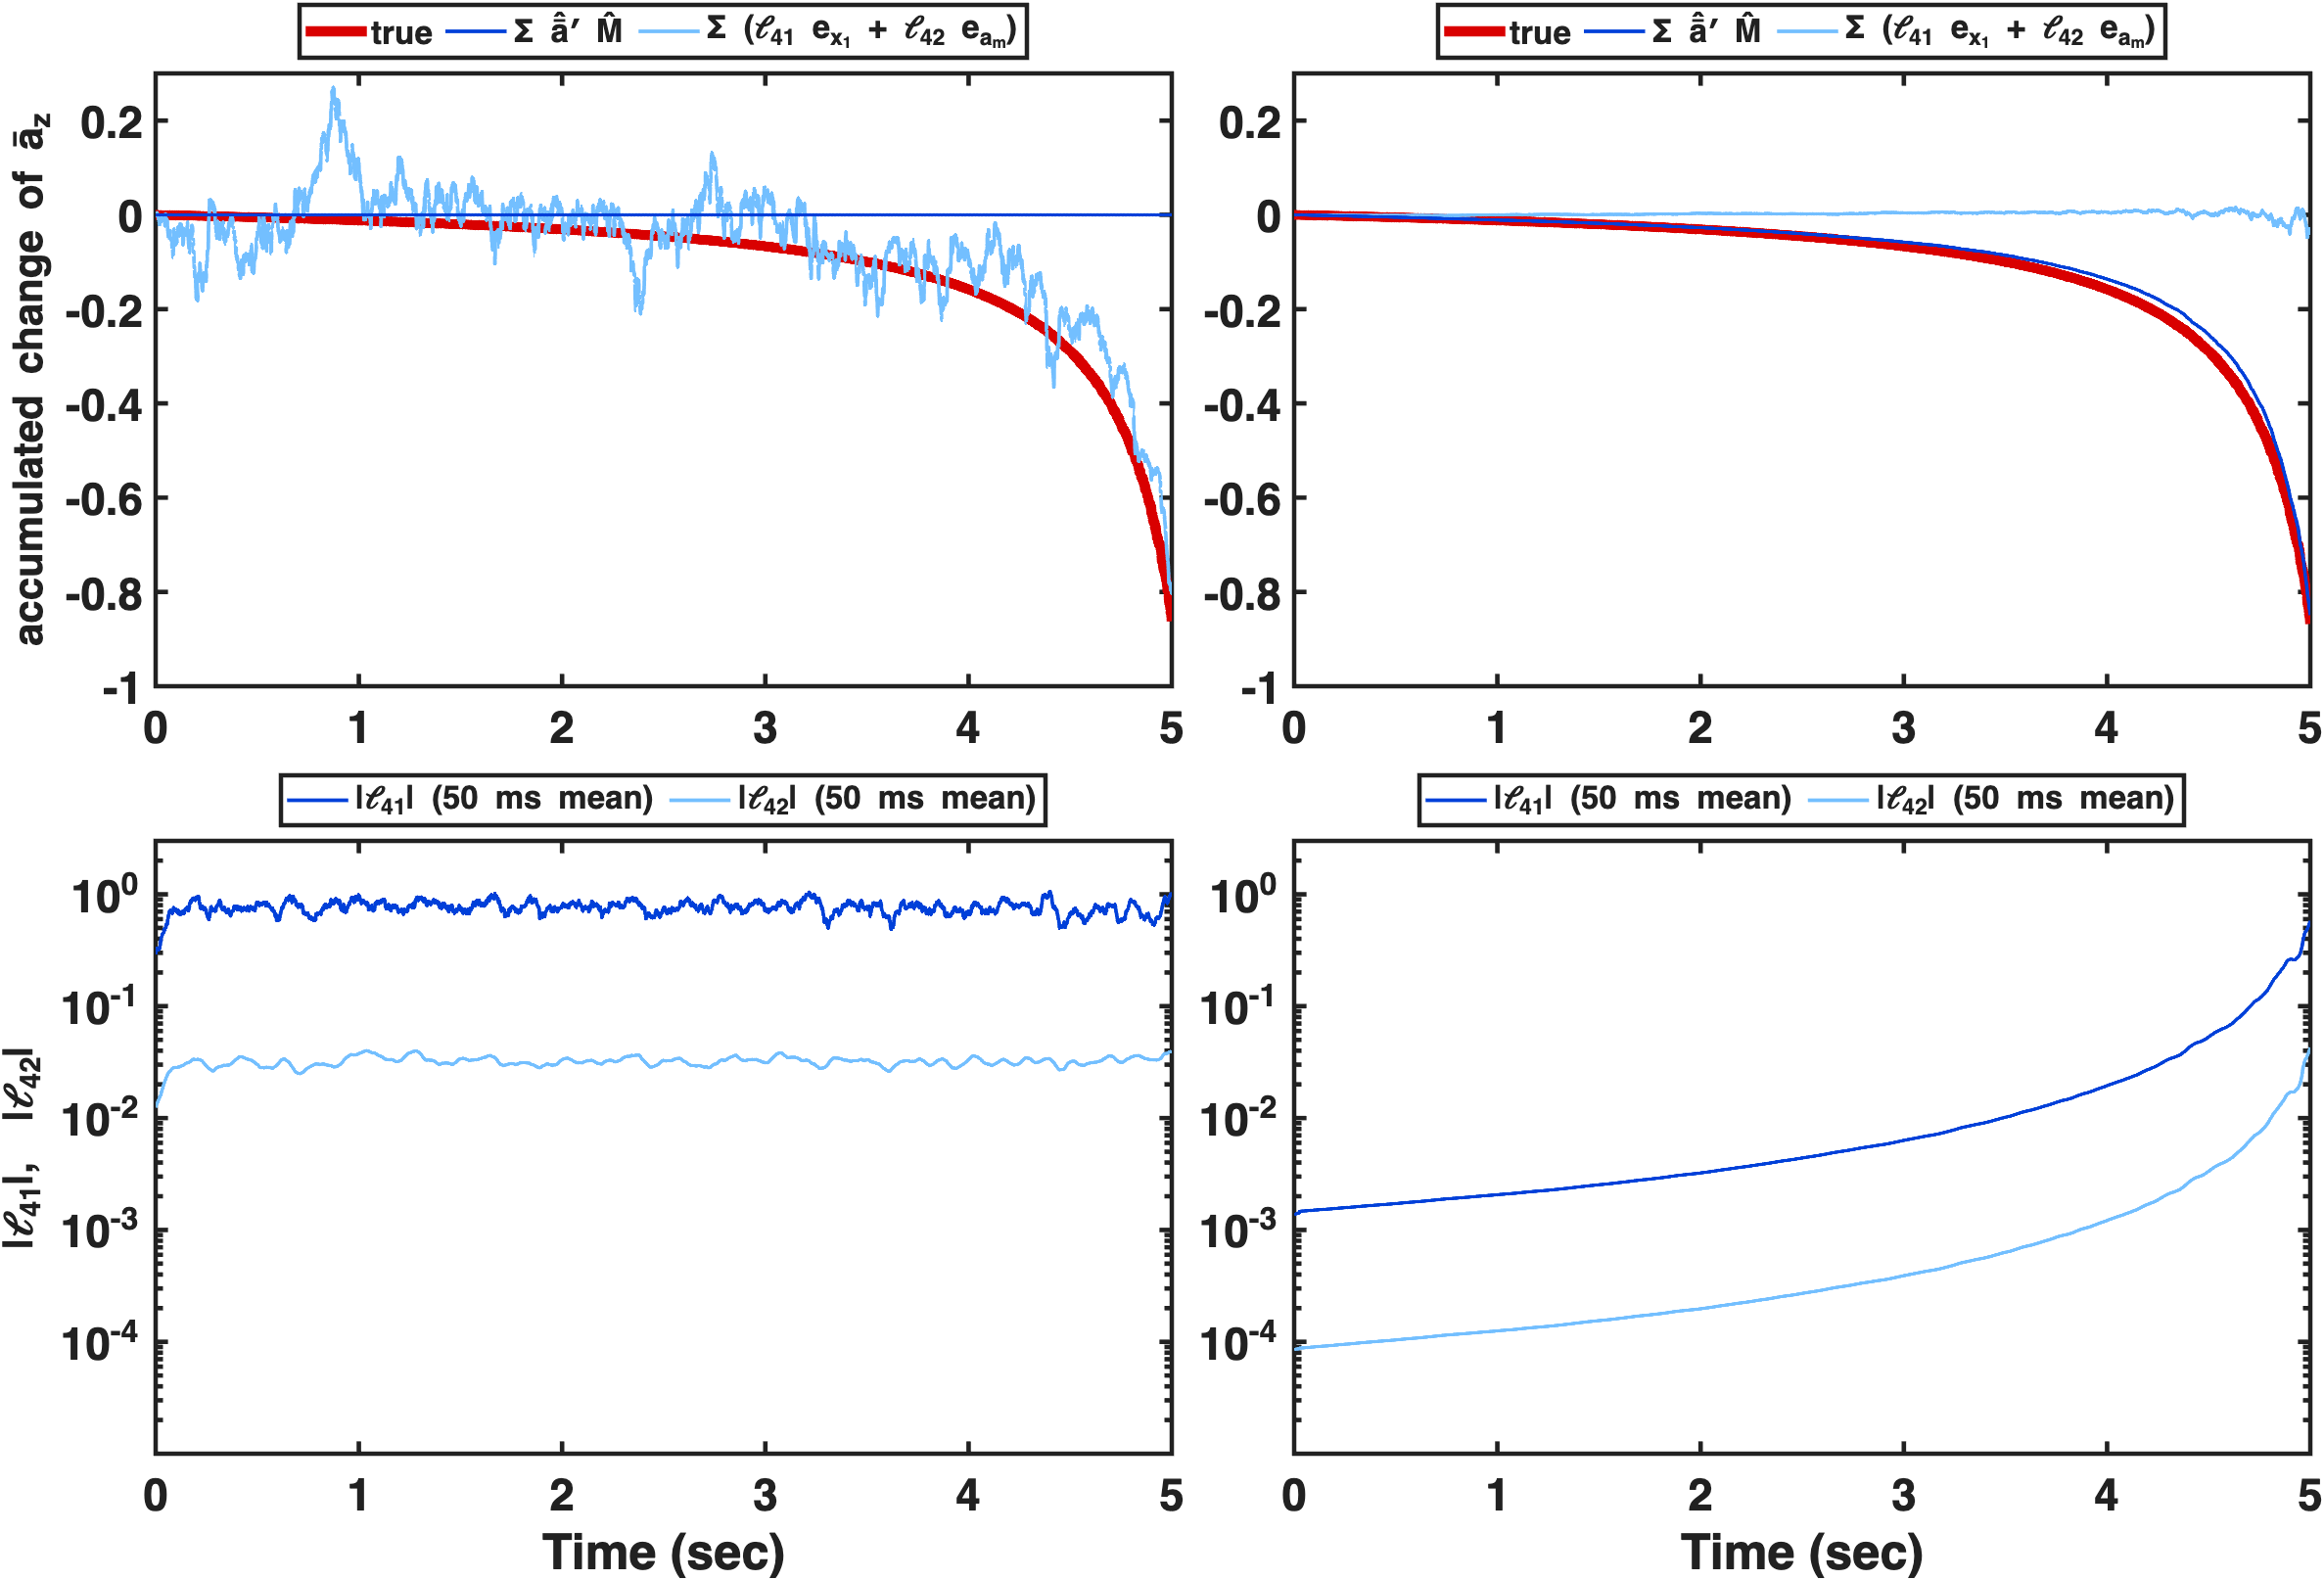
\includegraphics[width=\textwidth,height=0.68\textheight,keepaspectratio]{fig_mc_s5_split_s1.png}\end{center}
\figpage{Fig.~5.3\quad First order vs position-dependent motion gain: oscillation}{z axis; trajectory of Fig.~4.3 (triangle 1.10 $\leftrightarrow$ 10 R, 2 Hz); left: Section 4 estimator; right: this section, $q_{55} = 0$; plane wall, $\lc = 0.4$, seed 1}{fig_mc_s5_tri_s1.png}

% Section 6 of motion_ctrl.tex (Layer-1 session, 2026-10-07): unknown wall type, process noise of c (q55 = P_fix^2 I).
%   Replaces part2_conly.tex (kept on disk). The estimator of Section 5 unchanged; the wall type is given to the plant only and
%   the estimator starts from the plane values on every wall (.claude/rules/wall-test-protocol.md). c-hat is not shown here
%   (user 10-07, revised: c-hat shown in Section 6 with the wall's c(h_d) = 1 - h_d^2 a'(h_d) as the true value).
%   Seed of c = 0 on every wall (user 10-07; before: the plane band fit 0.0533); sqrt(p55[0]) = 0.1 (opts.sig). With P_fix the
%   results did not change at 3 decimals (the start value is forgotten before the near-wall band); q55 = 0 changed < 0.003. a_hat[0] = plane polynomial at the start height
%   (formC_b plaw_c_slope seed, local_law_delta).
%   Fig. 6.5 (user 10-07): ramp T_d then hold 0.2 T_d (run_mc_s5_conly 'rh050', P_fix; plot_mc_s6_walltype.m). T_d sweep, 5 seeds,
%   end-of-hold c-hat plane / cell: 0.5 s 0.12+-0.07 / 0.66+-0.10 (5.4 sd apart), 1 s 0.08 / 0.62 (4.1), 2 s 0.18 / 0.67 (2.9);
%   q55 = 0 separates 18 / 11 / 8 sd but cell sits at 0.36 (true c(1.10) = 0.74). T_d = 0.5 s chosen.
%   KF steps for c (user 10-07: as in the old part2, with the Section 5 H, which has no c column): l51, l52 through
%   p^f_51, p^f_54; p55 update; I[k]; forecast. Then the P_fix choice.
%   Plants: plane = production polynomial (calc_correction_functions.m, c_perp = 1/D_perp); cell = the same polynomial slid by
%   1.05 R (test_script/scratch/cell_cperp_delta.m, ledger C62).
%   Code: formC_b via run_plaw_walls law 'f1p2', q55_adapt 'ratio' (q55 = P_fix^2 I, single sqrt(P_fix) = 0.15; user 10-06:
%   one P_fix, no new/revisit split), production refinements ON and not shown. Runs: run_mc_s5_conly.m tags _mcs5_tri and
%   _mcs5_tri_ratio, plants plane and cell; figures plot_mc_s5.m 's6_plane' / 's6_cell', plot_mc_s6_a_of_h.m (Fig. 6.1), plot_mc_s6_c_of_h.m (Fig. 6.2).
%   Measured 10-07 (5 seeds, triangle 1.10 <-> 10 R at 2 Hz, e_a = a_true - a_hat): plane q55 = 0 troughs +0.022 tops +0.054,
%   P_fix troughs +0.005 tops +0.004 (mean |e_a| 0.039 -> 0.015); cell q55 = 0 troughs +0.075 tops +0.024, P_fix troughs +0.014
%   tops +0.012 (mean |e_a| 0.021 -> 0.019); dz_m rms plane 0.0292 -> 0.0271, cell 0.0269 -> 0.0265 um.
\clearpage
\section{Unknown wall type: process noise of $c$}

\hd{Motion gain of the two walls (plant only)}
\[
\begin{aligned}
D_\perp(u) &= 1 - \tfrac{9}{8}\,u + \tfrac{1}{2}\,u^{3} - \tfrac{57}{100}\,u^{4} + \tfrac{1}{5}\,u^{5} + \tfrac{7}{200}\,u^{11} - \tfrac{1}{25}\,u^{12} \\
\ba_{\mathrm{plane}}(h) &= D_\perp\Big(\frac{1}{h}\Big) \\
\ba_{\mathrm{cell}}(h) &= D_\perp\Big(\frac{1}{h + 1.05}\Big)
\end{aligned}
\]

\hd{Value of $c$ that makes the motion-gain slope exact at $h$}
\[
\ba'(h) = \frac{1 - c(h)}{h^{2}} \quad\Longrightarrow\quad c(h) = 1 - h^{2}\,\ba'(h)
\]

\hd{Feedback gain on $c$ (row 5 of $\mathbf{L}[k]$, $\mathbf{H}$ of Section 5)}
\[
\big[\,\ell_{51}[k],\ \ell_{52}[k]\,\big] = \big[\,p^f_{51}[k],\ p^f_{54}[k]\,\big]\,\big(\mathbf{H}\,\mathbf{P}^f[k]\,\mathbf{H}^T + \mathbf{R}[k]\big)^{-1}
\]

\hd{Update of $\hat{c}$ and of its variance}
\[
\begin{aligned}
\ch[k+1] &= \ch[k] + \ell_{51}[k]\,e_{x_1}[k] + \ell_{52}[k]\,e_{a_m}[k] \\
p_{55}[k] &= p^f_{55}[k] - \ell_{51}[k]\,p^f_{15}[k] - \ell_{52}[k]\,p^f_{45}[k]
\end{aligned}
\]

\hd{Information gained on $c$ at step $k$}
\[
I[k] = \frac{1}{p_{55}[k]} - \frac{1}{p^f_{55}[k]} \;\ge\; 0
\]

\hd{Forecast of the variance}
\[
p^f_{55}[k+1] = p_{55}[k] + q_{55}[k]
\]

\hd{Choice of $q_{55}$: constant variance $p^f_{55} = P_{\mathrm{fix}}$}
\[
\begin{aligned}
p^f_{55}[k+1] &= p^f_{55}[k] = P_{\mathrm{fix}} \\
q_{55}[k] &= P_{\mathrm{fix}} - p_{55}[k] \\
\frac{1}{p_{55}[k]} &= \frac{1}{P_{\mathrm{fix}}} + I[k] \\
q_{55}[k] &= \frac{P_{\mathrm{fix}}^{2}\, I[k]}{1 + P_{\mathrm{fix}}\, I[k]}
\end{aligned}
\]
\[
P_{\mathrm{fix}}\, I[k] \ll 1 \quad\Longrightarrow\quad \boxed{\,q_{55}[k] = P_{\mathrm{fix}}^{2}\, I[k]\,}
\]

\figpage{Fig.~6.1\quad Motion gain of the two walls}{$\ba_{\mathrm{plane}}(h)$ and $\ba_{\mathrm{cell}}(h)$; $h$ from 1.10 to 22.2 R}{fig_mc_s6_a_of_h.png}
\figpage{Fig.~6.2\quad Value of $c$ that makes the slope exact, $c(h) = 1 - h^{2}\,\ba'(h)$}{plane and cell; $h$ from 1.10 to 22.2 R}{fig_mc_s6_c_of_h.png}
\figpage{Fig.~6.3\quad Plane wall: $q_{55} = 0$ vs $q_{55} = P_{\mathrm{fix}}^{2} I$}{z axis; trajectory of Fig.~4.3; left: $q_{55} = 0$ (Section 5); right: $\sqrt{P_{\mathrm{fix}}} = 0.15$; $\lc = 0.4$, seed 1}{fig_mc_s6_plane_s1.png}
\figpage{Fig.~6.4\quad Cell wall: $q_{55} = 0$ vs $q_{55} = P_{\mathrm{fix}}^{2} I$}{z axis; trajectory of Fig.~4.3; left: $q_{55} = 0$; right: $\sqrt{P_{\mathrm{fix}}} = 0.15$; $\lc = 0.4$, seed 1}{fig_mc_s6_cell_s1.png}

\figpage{Fig.~6.5\quad Wall type read from $\hat{c}$ at the end of the descent}{z axis; 22.2 $\to$ 1.10 R in 0.5 s, then hold 0.1 s; $\sqrt{P_{\mathrm{fix}}} = 0.15$; left: plane wall; right: cell wall; $\lc = 0.4$, seed 1}{fig_mc_s6_walltype_rh050_s1.png}

% Section 7 of motion_ctrl.tex (Layer-1 session, 2026-10-07): reference result, raster scan parallel to the wall (user 10-07,
%   from a trajectory sketch: x 4 Hz triangle +-20 um = 320 um/s, y +1 um at every x turnaround, z held at 1.10 R).
%   Estimator: Section 6 on z (c-only, q55 = P_fix^2 I, sqrt(P_fix) 0.15, c[0] = 0); on x, y the flag par_wall_known of
%   motion_control_law_formC_b.m (10-07): the gain follows the plane's parallel law driven by the commanded wall-normal step only,
%   seeded at the plane's parallel gain. Without it the perpendicular slope times the axis's own tracking error was fed as a
%   gain step and a_hat_x hit the floor/ceiling (x tracking rms 1.05 um, offset +0.9 um; with it 0.020 um, offset 0.000 um;
%   flag off is bit-identical, verify_formC_b_production_defaults ALL PASS). Before/after: plot_mc_raster_x.m (not in the text).
%   Trajectory: trajectory_generator tan_shape = 1 (triangle) and tan_v_stair = 1 (staircase), amp_u = amp_v-step sign -1
%   because u_hat = -x, v_hat = -y in this frame. Run: run_plaw_walls tag _mcs5_raster110_ratio_parwk (5 seeds);
%   figures plot_mc_raster_ref.m ('traj', 'gain'). Seed 1: tracking rms x 0.020, y 0.019, z 0.0095 um; gains x 0.423 / 0.423,
%   y 0.423 / 0.426, z 0.087 / 0.091 (true / estimate, t > 0.5 s).
\clearpage
\section{Reference result: raster scan parallel to the wall}

\subsection*{Fig.~7.1\quad Raster scan: scan pattern and desired trajectory}\noindent{\small\textcolor[gray]{0.35}{left: $y$ vs $x$, actual (red) and desired (blue dashed); right: $x_d$ (4 Hz triangle, $\pm 20$ \textmu m), $y_d$ (+1 \textmu m at every $x$ turnaround), $z_d$ (held at 1.10 R); plane wall, $\lc = 0.4$, seed 1}}\par\smallskip
\begin{center}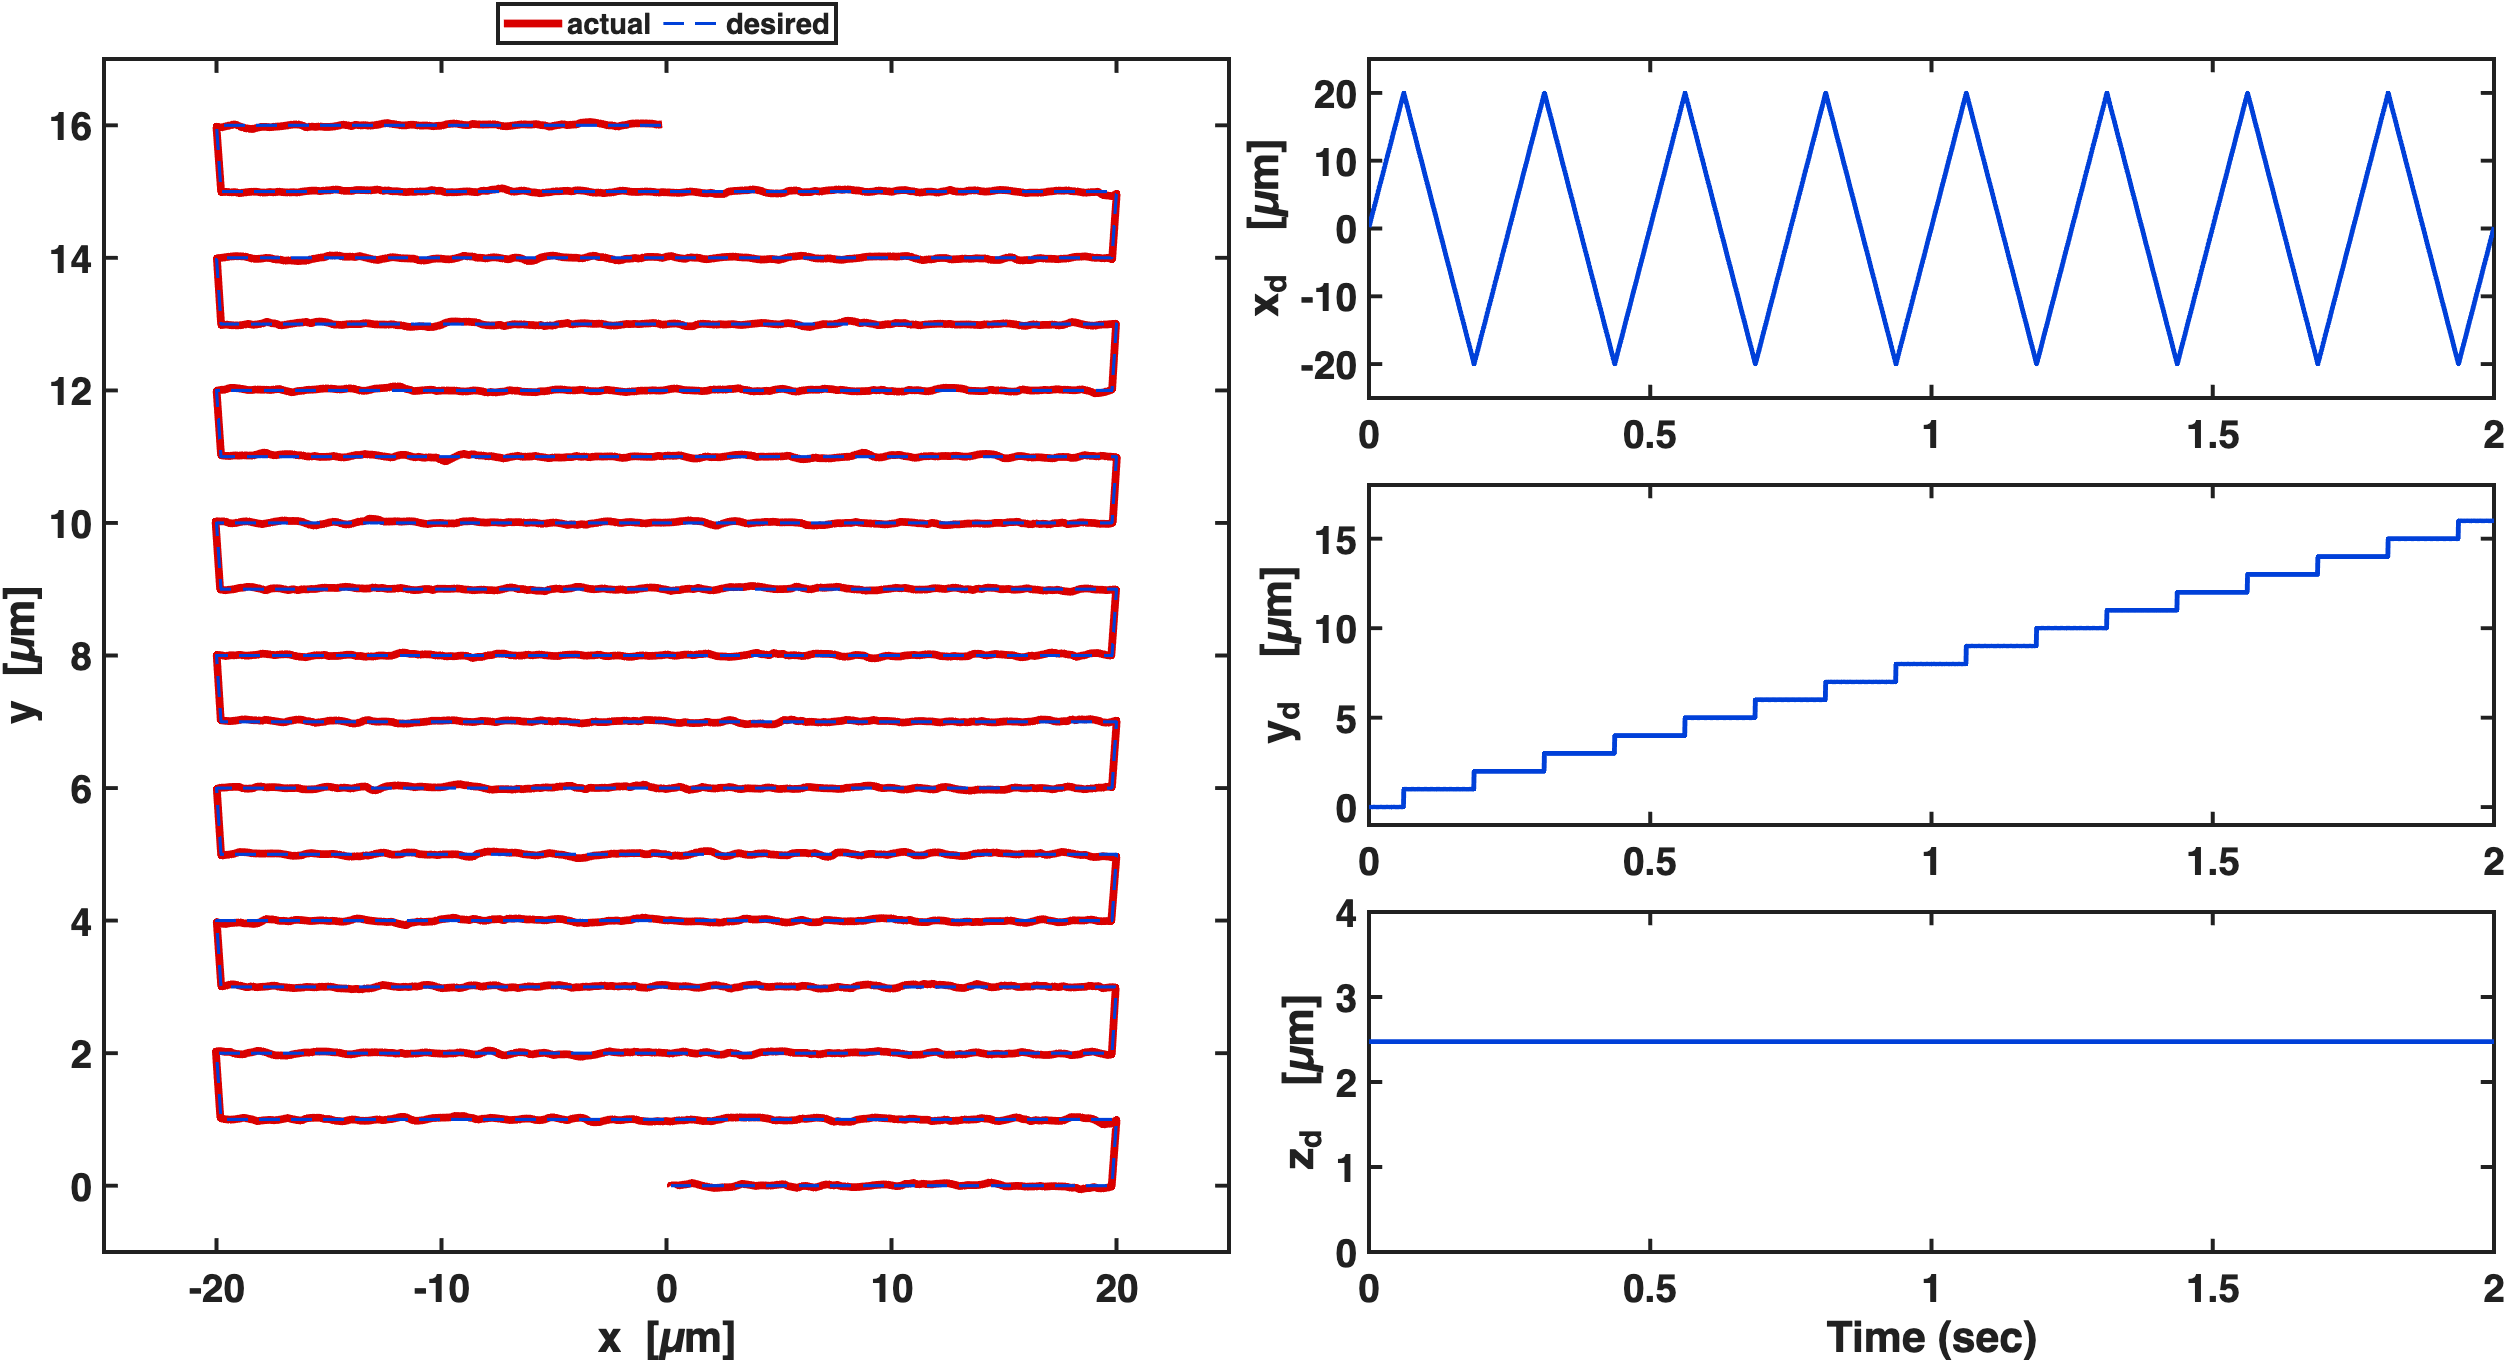
\includegraphics[width=\textwidth,height=0.72\textheight,keepaspectratio]{fig_mc_raster_traj_s1.png}\end{center}
\figpage{Fig.~7.2\quad Raster scan: motion gain and measured tracking error, three axes}{left: true (red) and estimated (blue) motion gain; right: measured tracking error; $z$: Section 6 estimator; $x$, $y$: plane parallel law driven by the wall-normal step; plane wall, $\lc = 0.4$, seed 1}{fig_mc_raster_gain_s1.png}

\ifdefined\mcshare\else% Appendix of motion_ctrl.tex: where each figure comes from. Regenerate all: test_script/scratch/make_motion_ctrl_figs.m
%   (runs are cached in test_results/temp_5state_noap and test_results/temp_plaw_walls; a missing cache file is re-run).
\clearpage
\section*{Appendix: figure provenance}

{\small
\begin{tabular}{@{}L{6.4cm}L{4.8cm}L{4.4cm}@{}}
\toprule
figure & plot script (\texttt{test\_\allowbreak{}script/scratch/}) & runs \\
\midrule
2.1 \texttt{fig\_\allowbreak{}mc\_\allowbreak{}s2\_\allowbreak{}traj} & \texttt{plot\_\allowbreak{}mc\_\allowbreak{}s2\_\allowbreak{}traj} & trajectory definition (no run) \\
2.2 \texttt{fig\_\allowbreak{}mc\_\allowbreak{}s2\_\allowbreak{}xyz} & \texttt{plot\_\allowbreak{}mc\_\allowbreak{}s2\_\allowbreak{}xyz} & \texttt{run\_\allowbreak{}mc\_\allowbreak{}s2\_\allowbreak{}xyz}: law with $\hat{\ba} = \ba$ or 1, $\lc = 0.4$, seed 1 \\
3.1 \texttt{fig\_\allowbreak{}mc\_\allowbreak{}s3\_\allowbreak{}am} & \texttt{plot\_\allowbreak{}mc\_\allowbreak{}s3\_\allowbreak{}am} & Section 2 run, $\hat{\ba} = \ba$, z axis \\
4.1 \texttt{fig\_\allowbreak{}mc\_\allowbreak{}s4\_\allowbreak{}eps\_\allowbreak{}s1} & \texttt{plot\_\allowbreak{}mc\_\allowbreak{}s4(1, 'eps')} & \texttt{run\_\allowbreak{}mc\_\allowbreak{}s4\_\allowbreak{}first\_\allowbreak{}order}, $\epsilon = 0$ vs $10^{-5}$, $\lc = 0.4$ \\
4.2 \texttt{fig\_\allowbreak{}mc\_\allowbreak{}s4\_\allowbreak{}nominal\_\allowbreak{}s1} & \texttt{plot\_\allowbreak{}mc\_\allowbreak{}s4(1, 'nominal')} & same runner, law with $\hat{\ba} = 1$ vs the estimate, three axes \\
4.3 \texttt{fig\_\allowbreak{}mc\_\allowbreak{}s4\_\allowbreak{}tri\_\allowbreak{}s1} & \texttt{plot\_\allowbreak{}mc\_\allowbreak{}s4(1, 'tri')} & same runner, \texttt{plain\_\allowbreak{}tri10}: 1 s descent, triangle 1.10--10 R, 2 Hz \\
5.1 \texttt{fig\_\allowbreak{}mc\_\allowbreak{}s5\_\allowbreak{}desc\_\allowbreak{}s1} & \texttt{plot\_\allowbreak{}mc\_\allowbreak{}s5(1, 'desc')} & \texttt{run\_\allowbreak{}mc\_\allowbreak{}s5\_\allowbreak{}conly} + Section 4 \texttt{prod\_\allowbreak{}xyz}, $q_{55} = 0$ \\
5.2 \texttt{fig\_\allowbreak{}mc\_\allowbreak{}s5\_\allowbreak{}split\_\allowbreak{}s1} & \texttt{plot\_\allowbreak{}mc\_\allowbreak{}s5\_\allowbreak{}split} & Fig.~5.1 runs; split as \texttt{probe\_\allowbreak{}mc\_\allowbreak{}s5\_\allowbreak{}update\_\allowbreak{}split} \\
5.3 \texttt{fig\_\allowbreak{}mc\_\allowbreak{}s5\_\allowbreak{}tri\_\allowbreak{}s1} & \texttt{plot\_\allowbreak{}mc\_\allowbreak{}s5(1, 'tri')} & same, triangle 1.10--10 R, 2 Hz \\
6.1 \texttt{fig\_\allowbreak{}mc\_\allowbreak{}s6\_\allowbreak{}a\_\allowbreak{}of\_\allowbreak{}h} & \texttt{plot\_\allowbreak{}mc\_\allowbreak{}s6\_\allowbreak{}a\_\allowbreak{}of\_\allowbreak{}h} & plant laws only (no run) \\
6.2 \texttt{fig\_\allowbreak{}mc\_\allowbreak{}s6\_\allowbreak{}c\_\allowbreak{}of\_\allowbreak{}h} & \texttt{plot\_\allowbreak{}mc\_\allowbreak{}s6\_\allowbreak{}c\_\allowbreak{}of\_\allowbreak{}h} & plant laws only (no run) \\
6.3 \texttt{fig\_\allowbreak{}mc\_\allowbreak{}s6\_\allowbreak{}plane\_\allowbreak{}s1} & \texttt{plot\_\allowbreak{}mc\_\allowbreak{}s5(1, 's6\_\allowbreak{}plane')} & \texttt{run\_\allowbreak{}mc\_\allowbreak{}s5\_\allowbreak{}conly}, q55 none / ratio 0.15, plane \\
6.4 \texttt{fig\_\allowbreak{}mc\_\allowbreak{}s6\_\allowbreak{}cell\_\allowbreak{}s1} & \texttt{plot\_\allowbreak{}mc\_\allowbreak{}s5(1, 's6\_\allowbreak{}cell')} & same, cell, plane init \\
6.5 \texttt{fig\_\allowbreak{}mc\_\allowbreak{}s6\_\allowbreak{}walltype\_\allowbreak{}rh050\_\allowbreak{}s1} & \texttt{plot\_\allowbreak{}mc\_\allowbreak{}s6\_\allowbreak{}walltype} & \texttt{run\_\allowbreak{}mc\_\allowbreak{}s5\_\allowbreak{}conly('rh050', P\_fix)}, plane + cell \\
7.1 \texttt{fig\_\allowbreak{}mc\_\allowbreak{}raster\_\allowbreak{}traj\_\allowbreak{}s1} & \texttt{plot\_\allowbreak{}mc\_\allowbreak{}raster\_\allowbreak{}ref('traj')} & run\_plaw\_walls tag \_mcs5\_raster110\_ratio\_parwk \\
7.2 \texttt{fig\_\allowbreak{}mc\_\allowbreak{}raster\_\allowbreak{}gain\_\allowbreak{}s1} & \texttt{plot\_\allowbreak{}mc\_\allowbreak{}raster\_\allowbreak{}ref('gain')} & same run \\
\bottomrule
\end{tabular}
}

\smallskip
{\small all runs: \texttt{run\_plaw\_walls} law \texttt{f1p2}, \texttt{sig} 0.10, plane init; plants plane and cell (\texttt{cell\_cperp\_delta}).}
\fi

\end{document}
